\chapter{System Architecture}     
        This chapter goes into the detail about the system components and their connections as a whole.
        The system architecture organizes the system's necessities into manageable blocks as shown in figure \ref{fig:systemstructure}.
        It is essentially divided into two major components, the Social Routing Client Application \cite{clientapplicationdocs} and the Social Routing Service with a third one being the external services.
        
        \vfill
        \begin{figure}[h]            
            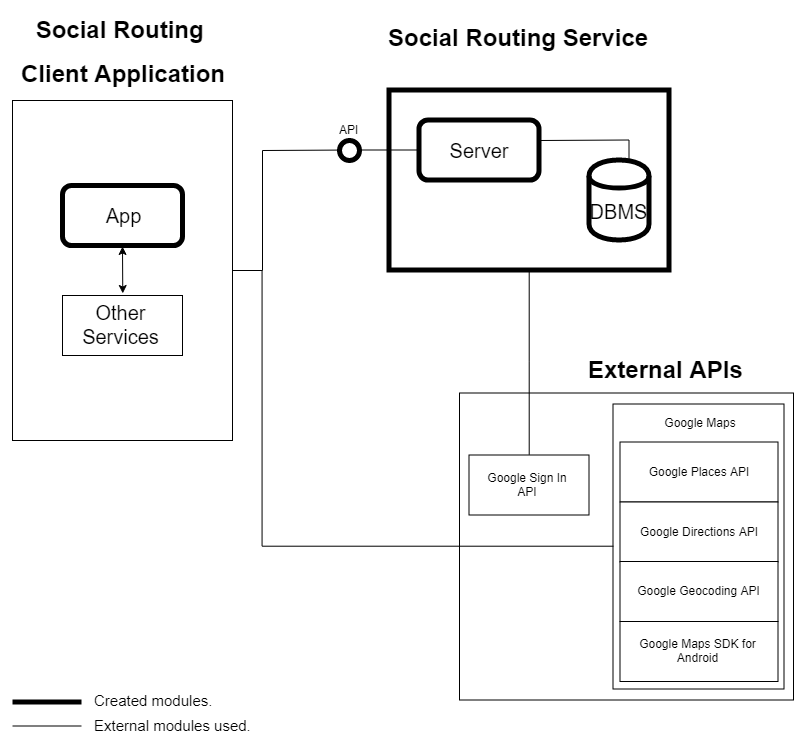
\includegraphics[width=\textwidth]{images/project-structure/system-structure.PNG}
            \caption{System structure.}
            \label{fig:systemstructure}
        \end{figure} 

        The Social Routing Service is subdivided into two components, the Server and the Database Management System\cite{dbmsdefinition}. The Server exposes its
        functionality through an HTTP\cite{httponlinedocs} API\cite{api} (Social Routing API \cite{apidocs}) and as such, receives requests from a client, processes the received request and responds accordingly.
        The Database Management System is used to store the server's data, over which the necessary calculations are made. 
        The Social Routing Service uses only one external API, Google Sign In\cite{googlesignindocs}, which is used to help with user authentication.

        The role of the Social Routing Client Application is to provide an interface to Android \cite{androiddocs} devices which the user can interact with, to expose the project 
        idea and essentially to demonstrate the Social Routing Service functionalities to the client. This component communicates with the Social Routing Service and 
        external services when required, through the HTTP protocol. The external services are APIs provided by the Google Maps platform \cite{googlemapsplatform} 
        to retrieve information such as the user profile from google accounts and content that helps managing the the Google maps, like locations, places and routes. 

        To authenticate a user in the system every component has a role, and because of it the general
        logic of authentication is part of the system's description. The figure \ref{fig:authenticationdiagram} describes the authentication logic in
        the project's scope.
        \newpage
        
        \section{System authentication}
        \vspace{-\baselineskip}
        \begin{figure}[h]            
            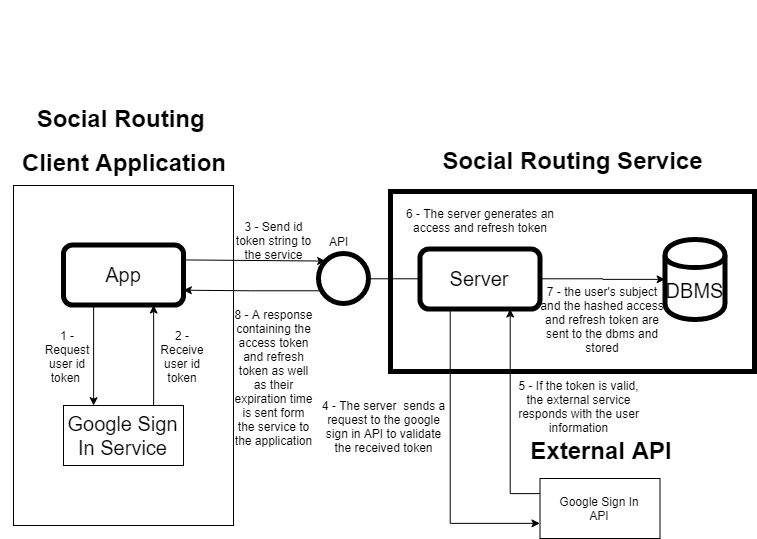
\includegraphics[width=\textwidth]{images/project-structure/authentication-diagram.PNG}
            \caption{Authentication diagram.}
            \label{fig:authenticationdiagram}
        \end{figure} 
        The authentication process begins with a request from the Client Application for the user id token, obtained through a Google Sign In internal service.
        The received id token string is then sent in an HTTP Post request to the API, to try and obtain service authentication credentials.
        When the service receives the token it must verify it's authenticity and for that a request is made to an external API Google Sign In, that
        upon correct token validation responds with user related information of which the subject is part of. After the token validation is complete
        the server then generates an access and a refresh token, which it then hashes and sends to the database along with the retrieved subject. 
        This information is stored to allow that in the future the user does not need to request credentials if they are already in his possession.
        After the storing process is complete a response is sent to the Client Application containing the generated access token and refresh token
        which will then be used to make authenticated requests to the server. 
